\documentclass[margin={3pt 0 0 0}]{standalone}
\usepackage{tikz,xcolor-material}
\begin{document}
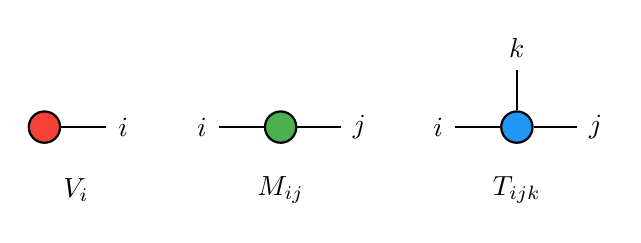
\begin{tikzpicture}[inner sep=4pt, thick]
  \path node (V)  at (  0,0) [circle, draw, fill=MaterialRed] {}
        node (Vi) at (  1,0) {$i$}
        node (M)  at (  3,0) [circle, draw, fill=MaterialGreen] {}
        node (Mi) at (  2,0) {$i$}
        node (Mj) at (  4,0) {$j$}
        node (T)  at (  6,0) [circle, draw, fill=MaterialBlue] {}
        node (Ti) at (  5,0) {$i$}
        node (Tj) at (  7,0) {$j$}
        node (Tk) at (  6,1) {$k$}
        node at (.4,-.8) {$V_i$}
        node at ( 3,-.8) {$M_{ij}$}
        node at ( 6,-.8) {$T_{ijk}$};
  \draw (V) -- (Vi)
        (M) -- (Mi) (M) -- (Mj)
        (T) -- (Ti) (T) -- (Tj) (T) -- (Tk);
\end{tikzpicture}
\end{document}
